
% ----------------------------------------- %
\chapter{統計処理の応用;高エネルギー実験}
% ----------------------------------------- %

高エネルギー素粒子実験では、未知の素粒子の兆候を掴むために様々な測定を行っている。
新しい物理模型が存在すればこの様な兆候として発見することができる、という事前の調査に基づいて研究を進めていく。
信号事象として新粒子の兆候、背景事象として既存の理論に起因する兆候を割り当てて考えていくことが多い。
新粒子の発見が勿論究極の目標であるが、そこに至るまでの過程で様々な理論模型を棄却して可能性のある領域を絞っていく作業も
非常に重要である。
高エネルギー実験ではこれらを統計処理で発見・棄却の評価を行っていくが、通常の検定とは少し毛色が異なるため独立した章として、
本章でその概要と詳細について議論する。

\section{はじめに}

高エネルギー実験では仮定する新物理事象から予測される兆候を掴むために、粒子のエネルギーや角度情報を測定する。
例えばヒッグス粒子であれば、粒子の不変質量を計算することで($H\to \gamma\gamma$などの反応)125GeV付近にピークを持つ不変質量分布を観測することができる。
また、ヒッグス粒子の反応とは全く関係のない2光子で不変質量を組んでしまうことも予想される。
そのため、得られる不変質量分布としては背景事象(ここでは標準理論で予想される通常の反応過程)の分布の上に、ピークが乗った様なヒストグラムを描くことができる。
実験屋としては、そのピークの幅(分解能)を絞るための手法の開発・改良を行ったり、背景事象をいかに削減するか・信号事象を
いかに無駄なく取得するかに工夫を凝らしていく。
そのうえでピークが見つかれば「発見」という結論となる。

問題は、背景事象から計算した分布が偶然125GeVにピークを持っただけではないのか、等どのような確率の上に成り立っていることであるかを
評価していく必要がある。

素粒子実験では目当ての事象をカウントして、そのカウント数$s$で理論モデルの検証を行っていく。
その際には背景事象もあるカウント数$b$だけ含まれてしまうことから、たとえ信号事象を観測できたとしてもノイズに埋もれてしまったら発見にはつながらない。
そこで、最終的には$b$に対して$s$が優位に大きいかどうかを議論する必要があるのだが、この手法にはいくつかの種類があり

\begin{itemize}
  \item カウンティング
  \item シェイプフィット
\end{itemize}

が主な手法である。大層な名前がついているが特に難しいわけではないのでじっくり考えれば理解できるはず。
信号の発見を行うには、$s=0$の仮説の$p-value$を計算することが一般的である。

これは、目的の新物理は世の中に存在しない場合($s=0$)に、実験で得られたイベント数がどれくらい普通に起きるかの目安となる。

\section{検定について}

\ref{}で述べた検定について、再度確認を行う。
ここでは帰無仮説$H_0$として「信号事象は存在する」を選択し、対立仮説として「信号事象は存在しない、背景事象で世の中は記述される」
を選択する。
しかし帰無仮説が棄却されたからといって、直ちに仮定する信号事象が存在する、という結論にはならない。

\section{p-value}

\begin{equation}
  p = \int_{\alpha}^{\infty} f(x)dx
\end{equation}

例えばガウス分布であれば、p値が小さければ小さいほど起こり得ない事象であると理解できる。
高エネ業界では専ら、p値を標準化された正規分布におけるsignificance $Z$ に焼き直して議論する。
\begin{equation}
  Z = \Phi^{-1}(1-p)
\end{equation}
$p=0.5$のときに$Z=0$、$p=0.05$のときに$Z=1.64$、$p=2.9\times 10^{-7}$の時$Z=5$となる。
つまり、標準化された正規分布の平均値から何$\sigma$離れた場所に位置しているかの指標となる。

\section{$S/\sqrt{B}$の導出}
背景事象$B$に対して信号事象$S$がどれだけ優位に多いかを表す指標であり、発見感度の議論の仕方としては最も基本的なものの一つである。
ポワソン分布の平均値$\lambda$が大きいときにガウス分布で近似できる性質を使う。
素粒子実験においてポワソン分布の平均値とは、「実験で観測できるとされる事象数 $s+b$」を意味する。
ゆえに十分な統計を溜めることのできる実験では以下の近似式を用いることができる。

\begin{equation}
  f(x)
  = \frac{1}{\sqrt{2\pi}\sigma} e^{\frac{(x-\mu)^2}{2\sigma^2}}
  = \frac{1}{\sqrt{2\pi(s+b)}} e^{\frac{{x-(s+b)}^2}{2(s+b)^2}}
\end{equation}

ここでポワソン分布は、 $\mu = s+b$、$\sigma = \sqrt{s+b}$
のパラメータを持つガウス分布で記述されている。

この近似式を用いた場合に、信号事象がゼロの仮説(background only hypothesis)に対するp値は次のように計算できる($s=0$)。

\begin{equation}
  p = 1 - \Phi \left(\frac{x-\mu}{\sigma} \right) = 1 - \Phi \left(\frac{x-b}{\sqrt{b}} \right)
\end{equation}

ここから、予想されるsignificance を求めることができて、
\begin{equation}
  \Phi \left(\frac{x-b}{\sqrt{b}} \right) = 1-p \\
\end{equation}

\begin{equation}\label{eq:signigicance_Z}
  \frac{x-b}{\sqrt{b}} = \Phi^{-1} (1-p) = Z
\end{equation}

(\ref{eq:signigicance_Z})式より、$x=s+b$の場合に予想されるsiginificanceは、

\begin{equation}
  \mathrm{med}[Z|s] = \frac{s}{\sqrt{b}}
\end{equation}

この式は信号事象の優位性を議論する時に広く用いられているものである。

\begin{figure}[h]
  \centering
  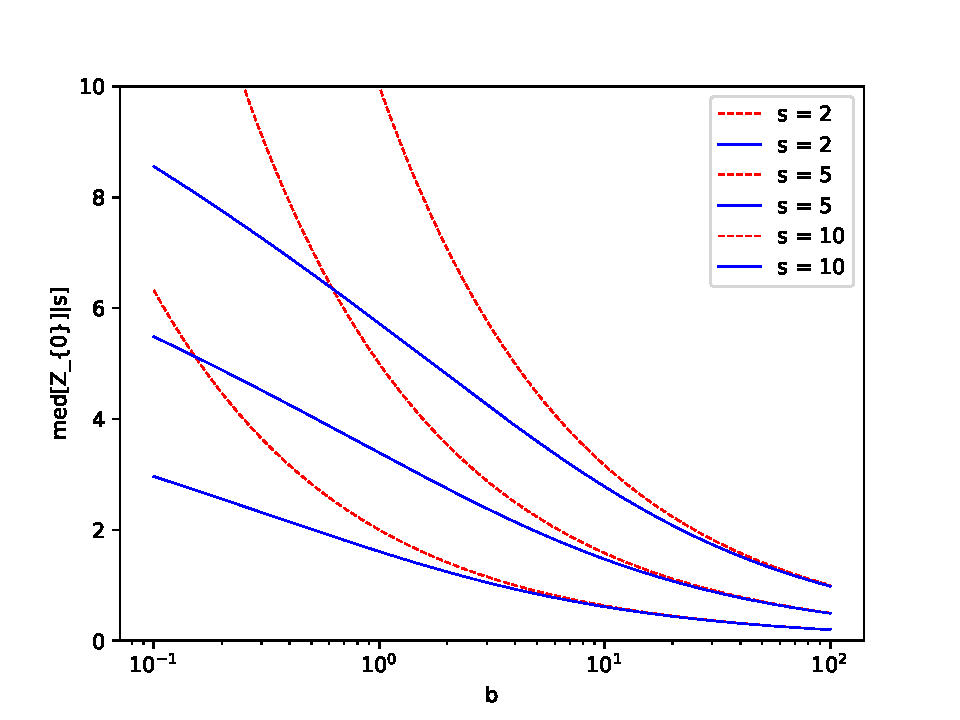
\includegraphics[scale=0.8]{python/discovery_significance.pdf}
  \caption{予想されるsiginificanceの分布。
  赤線は$Z=s/\sqrt{b}$、青線は$Z=\sqrt{2\left((s+b)\log\left({1+\frac{s}{b}}\right)-s\right)}$から見積もった曲線。
  Asimov siginificanceの方が背景事象が少なくなってくる領域でも正しくexpected limitを見積もることが可能である。
  基本的には$s/\sqrt{b}$はそのような領域ではoverestimationになっているだけで、$s/\sqrt{b}$同士で比較する分には多少の意味はある。
  }
\end{figure}


\section{Statistical test}

\begin{equation}
  \lambda(s) = \frac{L(s,\hat{\hat{\theta}}(s))}{L(\hat{s},\hat{\theta})}
\end{equation}


\section{Asymptotic formulae}
\subsection{導入}
ある確率変数$x$を測定して$N$ビンのヒストグラムを作成した($n_1,n_2,...,n_N$)。
$i$番目のビン内のイベント数の期待値は次のように表される。
\begin{equation}
E[n_i] = \mu s_i + b_i
\end{equation}
ここで$s_i$と$b_i$は$i$番目のビンにおける信号数と背景事象数の平均値である。
\begin{eqnarray}
 s_i = s_{tot}\int_{\mathrm{bin}~i}f_s(x;\theta_s)dx \\
 b_i = b_{tot}\int_{\mathrm{bin}~i}f_b(x;\theta_b)dx
\end{eqnarray}
$f(x;\theta)$は各モデルの確率密度関数を表しており、積分することで注目するビンに事象が得られる確率を計算することができる。また、$\mu$は信号強度であり、$\mu=0$の時にはbacground only hypothesis、$\mu=1$のときには信号を含んだ仮説を表現することができる。
$\theta$は確率密度関数の形状を決めるパラメーターで、$(\theta_s,\theta_b,b_{tot})$をまとめてnuisance parameter として扱う。

\subsection{likelihood}
作成したヒストグラムに対する尤度関数は、とあるビンに事象が観測される確率(ポワソン分布)の積で表すことができる。
\begin{equation}
    L(\mu, \theta) = \Pi_{\j=1}^{N} \frac{(\mu s_j + b_j)^{n_j}}{n_j!}e^{-(\mu s_j + b_j)}
\end{equation}
さらに、control regionを定義した解析では、CRにおける尤度関数も式に含めることができる。

\subsection{Profile likelihood ratio}
信号強度$\mu$を試験するために、profile likelihood ratio $\lambda(\mu)$を用いる。
\begin{equation}
  \lambda(\mu) = \frac{L(\mu,\hat{\hat{\theta}})}{L(\hat{\mu},\hat{\theta})}
\end{equation}
分母はLikelihoodの最大値、分子は$\mu$をとある値に固定した時にLikelihoodが最大となるように求めた$\theta$を用いたときの値。
尤度関数を最大にするパラメータの組み合わせは$(\hat{\mu},\hat{\theta})$であるため、常に分子は分母より小さいか分母に等しくなるので、$0<\lambda<1$が成り立つ。
$\lambda=1$はデータと$\mu$がよく一致することを表していて、0に近づくほど実験データと乖離している($\mu$を仮定した理論では実験データを説明できない、棄却される対象となる)ことが表される。

\subsection{test statistic $t_\mu=-2\ln\lambda$}
statistical testを行う際には、$\lambda$をさらに次の様に変換して用いることが多い。
\begin{equation}
  t_\mu=-2\ln\lambda(\mu) = -2 \left(\ln L(\mu,\hat{\hat{\theta}}) -  L(\hat{\mu},\hat{\theta} ) \right)
\end{equation}
先程の$\lambda$の範囲の議論より、$t_\mu$は$-2<t_\mu<0$の範囲を動く。
よって0に近いほど(値が大きくなるほど)、データと$\mu$の整合性が取れないことを表している。
\begin{equation}
p_\mu = \int_{t_{\mu,obs}} ^{\infty} f(t_\mu|\mu) dt_\mu
\end{equation}
$t_{\mu,obs}$は実験データから見積もった値、$f(t_\mu|\mu)$は$t_\mu$が得られる確率密度関数を表している。

\subsection{Test statistics $t_\mu$ for $\mu > 0$}
一般的に信号モデルは、既存のモデルに対してさらに数イベント信号が観測できると予測する。
そのため信号強度は正の値をとる。その場合を試験量も記述しておく。$\mu>0$の領域では今まで通りのlikelihood ratioを用いて、0以下の領域では$\mu$の値を0に固定したlikelihood ratioを定義しておく。

\subsection{Test statistics $q_\mu,q_0$}
高エネ実験では新物理$\mu=1$を探している。
実際の統計処理では$\mu=0$のbackground only hypothesisを棄却する方向で計算を進めていく\footnote{ここが少し混乱の元。示したいのは信号を含んだモデルが存在することであるが、統計処理では「信号を含まないモデル$H_0$では実験データを説明できない$\to$新しいモデルが必要となる」というロジックで進んでいく。}。
よって方針は、$\mu=0$のtest statisticsを正しく評価していくこととなる。
(で、問題は)ここから定義した$t_\mu$をさらにいろいろ条件を変えたときの式として、$q_\mu$に置き換えて議論していくので、本書もそれに倣う\footnote{
式の形は$t_\mu$の議論の時に示したとおりだが、$q_\mu$と明記したときには「$\mu$の値に関して条件を掛けて立式していきますよ」という意思表示だと思ってもらえればいい。}。

\begin{equation}
  q_0 = -2\ln\lambda(0) : \hat{\mu} > 0
\end{equation}
\begin{equation}
  q_0 = 0 : \hat{\mu} < 0
\end{equation}

\begin{equation}
  q_\mu = -2\ln\lambda(\mu) : \hat{\mu} < \mu
\end{equation}
\begin{equation}
  q_\mu = 0 : \hat{\mu} > \mu
\end{equation}

\section{Profile likelihood ratio の近似式}
信号強度$\mu$を試験する場合を考え、データ点は$\mu'$に従って分布しているとする。
\begin{equation}
-2\ln\lambda(\mu) = \frac{(\mu-\hat{\mu})^2}{\sigma^2} + O(1/\sqrt{N})
\end{equation}
ここで、$\hat{\mu}$はmean $\mu'$、標準偏差$\sigma$のガウス分布に従う。$N$はサンプル数を表す。
$\sigma$は共分散から簡単に求めることができて、
\begin{equation}
  V_{ij} = \mathrm{cov}[\hat{\theta_i}, \hat{\theta_j}]
\end{equation}

\section{カウンティング(1ビンフィット)}
ポワソン分布に従う事象を$n$事象観測して、1ビンのヒストグラムで評価する場合を考える。
SRにおける期待値は
\begin{equation}
E[n] = \mu s + b
\end{equation}
$s$は信号モデルから予想される信号事象数の平均値、$b$は背景事象数の期待値、$\mu$は信号強度を表す。
$b$はnuisance parameter \footnote{nuisanceとは迷惑なこと、厄介なこと、の意味を持つ単語。高エネの人が真に興味があるのは信号数なので、まぁ背景事象数は邪魔だということか。}であり、CRにおける背景事象数の分布から制限をかけることができる。
CRにおける背景事象の期待値は、SRとCRにおける背景数の違いを表す scale factor を$\tau$で表すと、
\begin{equation}
E[m] = \tau b
\end{equation}
と記述することができる。
実際の解析ではこの$\tau$もnuisance parameterとしてフィットから求める手順を踏むが、
ここでは簡単のために既知の値として話を進める。

実験から得られる値はSRの事象数$n$、CRにおける自少数$m$、興味のあるパラメータ(parameter of intereset; POI)$\mu$、そしてnuisance parameter $b$である。
ポワソン分布に従うような場合に、$\mu$と$b$に対して実験結果から次のような尤度関数を定義することができる。


\section{シェイプフィット}
1ビンではなく、分布の形を反映した統計処理を行いたい場合、こちらの手法を用いる。
俗語的に
\begin{itemize}
  \item シェイプフィット
  \item シェイプでフィットした
\end{itemize}
とか呼ばれる。

\section{CLs法}
以下で定義する$CL_s$と呼ばれる量をtest statisticとして用いて解析感度を評価する手法。

\begin{equation}
CL_s = \frac{CL_{s+b}}{CL_b}
\end{equation}

$CL_{x}$はたどっていくと$\mu$に依存する。
よく用いられるのは95$\%$CLsであり、$CL_s=0.05$となる$\mu$の値を探してそれを$\mu_{up}$として
解釈し、最終的に断面積の上限値設定に使用する手法である。


\chapter{高エネルギー実験における統計処理}

\section{Likelihood}
私達が興味のあるパラメータは(究極的には)信号事象の数に相当する信号強度$\mu$である。
自然界では既に$\mu$は定まった値を持っており、それを人間が知らないだけである。
そのため実験データが得られる確率は
\begin{equation}
P(\rm{data}|\mu)
\end{equation}
と表すことができる。
実験屋が持っている情報は実験データ(とシミュレーションサンプル)であり、データから確率密度関数を求める必要がある。
これがLikelihoodの意味するところである。
\begin{equation}
L(\mu)
\end{equation}

Likelihood 関数を用いると、信号強度$\mu$の推定も最大尤度法(Maximum likelihood; ML)を用いることで可能となる。
慣習的に推定量はハット記号で表し

\begin{equation}
\hat{\mu} = arg max L(\mu)
\end{equation}

と信号強度を推定することができる。
統計量が増加すると $\hat{\mu}\to\mu^{\rm{truth}}$ に近づく。

\subsection{Likelihoodを計算する}
実際の実験では例えば質量の分布(であったり、$p_T$、$E$であったり)のヒストグラムを計算して、
そこに背景事象とデータとの間に統計的に優位な乖離があるかどうかを判別することになる。つまり、

\begin{itemize}
  \item $H_0$:(この世の中には新物理などなく)データと背景事象は一致している
  \item $H_1$:(この世の中に新物理はある!)データと背景事象には何らかの乖離が生じている
\end{itemize}

とする2つの仮説を検討する、仮説検定の議論に持ち込むこととなる。
このときに Neyman-Pearsonの補題(検定量としてLikelihood ratioを用いるのが最も性能が良い)によると、
2つの仮説に基づいたLikelihood funcitonを計算して、それらの比を検定量とした仮説検定を行うことになる。
ヒストグラムに基づいたLikelihoodの計算方法には二種類ある。


\section{Likelihoodの使い方}

ヒストグラムさえ作ることができれば、あとは何らかのツール(もしくは手計算?)でlikelihoodを計算することができる。
計算したlikelihoodは主に3つの使い方が想定されている。

\subsection{Maximum likelihood parameter estimation}
\subsection{Frequentist confidence interval}
\subsection{Beysian credible interval}

\section{Profile likelihood}

あるビン$i$に期待される事象数は、

\begin{equation}
E(n_i) = \mu s_i + b_i
\end{equation}

で表される。$s_i$はそのビンに信号事象が何イベント存在するかを表しており、$b_i$は背景事象が何イベントあるかを表している。
よって$i$ビンに$n_i$事象観測される確率はポワソン分布を用いると

\begin{equation}
\mathcal{P} = \frac{(\mu s_i+b_i)^{n_i}}{n_i!}e^{-(\mu s_i+b_i)}
\end{equation}

と表される。全ビンに対して積を取るとLikelihood functionが定義でき

\begin{equation}
L(\mu)=\prod_{i\in bins} \frac{(\mu s_i+b_i)^{n_i}}{n_i!}e^{-(\mu s_i+b_i)}
\end{equation}

と表される。これが最も単純な形のLikelihood functionであり、$\mu$にのみ依存している。
これは信号事象も背景事象も完全に$100\%$その性質が分かっている実験(現実的にはありえないが)でのみ使用できるlikelihood関数である。\\

もちろん実際には$s_i$や$b_i$は系統誤差の影響(規格化定数や分布の形等の影響、実験家がコントロールできない影響)を受けるため、それらを表すパラメーター(nuisance parameter)として$\bm{\theta}$を用いて、

\begin{equation}
s_i \to s_i(\bm{\theta}),~~b_i\to b_i(\bm{\theta})
\end{equation}

と定義し直すと、likelihood は

\begin{equation}
L(\mu,\bm{\theta})=\prod_{i\in bins} \frac{(\mu s_i(\bm{\theta})+b_i(\bm{\theta}))^{n_i}}{n_i!}e^{-(\mu s_i(\bm{\theta})+b_i(\bm{\theta}))}
\end{equation}

と書き直せる(式の形としては何も変わっていないが)。
この様に、真に興味のある信号強度$\mu$以外のパラメーター(nuisance parameters;NPs)に依存させた likelihood を profile likelihood と呼ぶ。

\subsection{likelihood ratio}
検定量として profile likelihood を用いた尤度比を考える。

\begin{equation}
\lambda(\mu)=\frac{L(\mu,\hat{\hat{\bm{\theta}}})}{L(\hat{\mu},\hat{\bm{\theta}})}
\end{equation}

分子はある$\mu$の値に対してlikelihoodを最大にするNPの値$\hat{\hat{\bm{\theta}}}$を求めたlikelihoodである(confitional maximum-likelihood)。
また分母は全てのパラメーターをスキャンしてlikelihoodを最大にする値$\hat{\mu},~~\hat{\bm{\theta}}$を求めたlikelihoodである(unconditional maximum-likelihood)。
ゆえに定義から

\begin{equation}
0 < \lambda < 1
\end{equation}

の範囲を取る。


\subsection{系統誤差の扱い}
系統誤差は基本的には全く値のわからないものであり、別の実験ないし作業から求める必要がある。
つまり何らかの分布を使って「constrain」する必要がある。
Profile likelihoodは、系統誤差(systematics uncertainties)をlikelihood関数の中に含めることができる。
系統誤差は "constrained" nuisance parameter として式に含める。

\begin{equation}
L(n,\theta^0|\mu,\theta) = \prod_{i\in bins} \mathcal{P}(n_i|\mu \times S_i(\theta)+B(\theta)) \times \prod_{j\in syst} \mathcal{G}(\theta_j^0|\theta_j,\Delta \theta)
\end{equation}

ここで系統誤差は(慣習的に)平均値$\theta^0=0$、分散$\Delta \theta=1$の正規ガウス分布に従うものとされる。
系統誤差の影響とは、あるビン$i$に対して$+1$〜$-1$の値を取らせたときの影響を言う。

系統誤差がNuisance parameterとして尤度関数に含まれたように、
その他のパラメータも尤度関数に「free parameter」として含めることができる\footnote{free parameterとは、と思うかもしれないが値が実験から決めない変量のこと。例えば$\mu$はfree parameterで、尤度関数を最大にする値を推定値として取るという点で、$\mu$もfree parameterである。}。
この nuisance parameter を「Normalizatoin factors(NF)」と呼び、

\begin{equation}
B(\theta,k)=kB(\theta)
\end{equation}

の様に表現することができる($\mu S(\theta)$と同じ発想)。

\subsection{Fit}

もう一度系統誤差を含めたprofile likelihoodを眺めてみる。

\begin{equation}
L(n,\theta^0|\mu,\theta) = \prod_{i\in bins} \mathcal{P}(n_i|\mu \times S_i(\theta)+B(\theta)) \times \prod_{j\in syst} \mathcal{G}(\theta_j^0|\theta_j,\Delta \theta)
\end{equation}

このlikelihoodは$L(\bm{n},\bm{\theta}^0|\mu,\bm{\theta})$から分かるように、ある信号強度である系統誤差の値をとっている時に、データセット$\bm{n}$、系統誤差$\bm{\theta}^0$の値を取っている関数である。
事前に分かっているのはデータセット$\bm{n}$、系統誤差$\bm{\theta}^0$である\footnote{繰り返しになるが、慣習的にconstrain termのガウス分布は正規化されているので、$\theta^0=0$、$\Delta \theta=1$を意味している。そのため$\mathcal{G}(0|\theta,1)$として見ても良い。}。

maximum-likelihood estimationでパラメータ推定をした際には、
$(\mu,\theta_1,...,\theta_N )$の複数セットの推定量を計算することになる。

通常のlikelihoodは$\mu$に対する関数だったので、$\mu$をスキャンしていき尤度関数が最大値を取るところを見つければよかった。言い換えると一次元の関数の最大値を見つける問題に相当する。
対してProfile likilihoodは、nuisance parameterとして複数のfree parameterに依存しているので、
N次元の関数となっている。


\subsection{Likelihood ratio}
profile likelihood はこれまで見てきたようにNP(系統誤差、規格化定数etc)を含んでいる。
例えばある仮説(つまり$\mu$の値を何かに固定する、ex. $H_0$)を選んだ時に、どのNPの値を使えばよいのだろうか?
データに選ばせよう、というのがProfileの哲学である。

\begin{equation}
t_{\mu_0} =  -2 \ln\frac{L(\mu=\mu_0,\hat{\hat{\theta}})}{L(\hat{\mu},\hat{\theta})}
\end{equation}

を Profile likelihood ratio(PLR)と呼ぶ。

\begin{itemize}
  \item $\hat{\hat{\theta}}$は $\mu=\mu_0$に対するbest-fit(conditional MLE)
  \item $\hat{\theta}$はoverall (global)な best-fit (unconditional MLE)
\end{itemize}

Wilk's theoremによると、PLRは$\chi^2$分布に従うとされる。


% -------------------------------------- %
\chapter{Asimptotic Formulae}
% -------------------------------------- %

\section{物理探索における検定}

通常の検定と同様に帰無仮説と対立仮説を用意するが、どのような検定を行うかによって真逆の定義となる。

\begin{itemize}
  \item[discovering]\mbox{}\\
    \begin{itemize}
      \item $H_0$ : 背景事象のみとする仮説(background-only)
      \item $H_1$ : 背景事象+信号事象の仮説(signal + background)
    \end{itemize}
  \item[limit settting]\mbox{}\\
    \begin{itemize}
      \item $H_0$ : 背景事象+信号事象の仮説(signal + background)
      \item $H_1$ : 背景事象のみとする仮説(background-only)
    \end{itemize}
\end{itemize}

また通常の検定と同様に、実験データと仮説の合い具合は$p$-valueで評価される。

物理学において$p$-valueは、それと同値のsignificance $Z$に変換して議論を進めることが一般的である。
これは
\begin{equation}
    Z = \Phi^{-1}(1-p)
\end{equation}
と定義され、ガウス分布を用いた片側検定\footnote{物理学では信号事象があるかないか、つまり観測された実験結果が予想値よりも大きいかどうかを評価するため、右側の片側検定が通常である。}における累積分布関数に等しい。
例えばヒッグス粒子の「発見」の場合\footnote{先に導入した$H_0$と$H_1$の組み合わせに注意}、背景事象仮説$H_0$を$Z=5$の閾値以上で棄却している。
これは$p=2.87\times10^{^7}$に相当し、$H_0$を仮定した場合に実験結果が得られる可能性は非常に(非常に非常に)小さいことが分かる。
これがよく言う$5\sigma$で発見、という意味合いである。

ヒッグス粒子の例は「発見」についての考え方であったが、実験を稼働させる段階(もしくは前段階)において、
その実験が持つと期待される感度を正しく評価しておくことも重要である。




\chapter{Asimov data}

Likelihood ratioから計算した検定量(test statistics)は次の形をしていた。
\begin{equation}
  p_\mu = \int_{q_{\mu,\mathrm{obs}}}^\infty f(q_\mu|\mu)dq_\mu
\end{equation}
検定量のsampling distributionを知る必要がある。
上限値の設定のためには$f(q_\mu|\mu)$のがどのような分布になるかを事前に知っておく必要がある。
